\section{Frequency-domain subspace identification}
\label{sec:freq-doma-subsp}

This section describes a methods for estimation of the underlying linear
frequency response function and nonlinear coefficients for nonlinear systems.
The method is an (nonlinear) extension of linear subspace methods which are able
to deal with multiple-input, multiple-output(MIMO) systems.

The nonlinear subspace methods interpret nonlinearities as unmeasured internal
forces, ie. nonlinearities are seen as cause of distortion on the linear FRF
matrix. Two main nonlinear methods exist one in time domain, time-domain
subspace identification (TNSI)\autocite{marchesiello2008a}, and one in frequency
domain, frequency-domain subspace identification (FNSI)\autocite{noel2013a}.
\textit{N} denotes nonlinear.
Both performs equally well in identification and robustness, but the main
benefit of FNSI is that the input time series, when converted to frequency
domain, can be truncated to a frequency interval of interest and thus reduce the
computational time. FNSI is the method used here.


Given the equation of motion for a dynamical system with nonlinearities:

\begin{equation}
  \label{eq:EOM_fnsi}
  \bm M \ddot{\bm y}(t) + \bm C \dot{\bm y}(t) + \bm K \bm y(t) +
  \bm f_{nl} \left( \bm y(t), \dot{ \bm y}(t) \right) = \bm p (t)
\end{equation}

where $\bm M$, $\bm C$ and $\bm K \in \mathbb{R}^{n \times \, n}$ are the mass,
linear viscous damping and linear stiffness matrices; $\bm y(t)$ and $\bm p(t)
\in \mathbb{R}^{n}$ are the generalised displacement and external force vectors;
$\bm f_{nl}(t) \in \mathbb{R}^{n}$ is the essentially nonlinear restoring force
vector comprising elastic and dissipative contributions; $n$ is the number of
DOFs. Essentially nonlinear, or nonlinearisable, means that the function is zero
and have zero slope at the origin, i.e. it cannot be linearised.


The notation of \eqref{eq:EOM_fnsi} assumes that all linear components of the
restoring forces in the system are included in the matrices $\bm K$ and $\bm
C$. The nonlinear restoring force is expressed by a linear combination of $s$
lumped nonlinearities

\begin{equation}
  \label{eq:nonlin_fnsi_lummped}
  \bm f_{nl} \left( \bm y(t), \dot{\bm y}(t) \right) =
  \sum_{i=1}^s \mu_i \bm b_i \bm g_i \left( \bm y(t), \dot{\bm y}(t) \right)
\end{equation}
where $\mu_i$ is the unknown nonlinear coefficient and $\bm g_i \left( \bm y(t),
  \dot{\bm y}(t) \right)$ is the the corresponding known (characterised by eg.
WT or RFS) functional form (or basis function). The location of the nonlinearity
is specified by the boolean vector, $\bm b_i$.


Moving the nonlinear terms of \eqref{eq:EOM_fnsi} to the right-hand side

\begin{equation}
  \label{eq:EOM_fnsi_final}
  \bm M \ddot{\bm y}(t) + \bm C \dot{\bm y}(t) + \bm K \bm y(t) = -
  \sum_{i=1}^s \mu_i \bm b_i \bm g_i(t) + \bm p(t)
\end{equation}
the system may be viewed as the underlying linear system subjected to the
external force $\bm p(t)$ and the internal feedback force due to nonlinearities,
as shown in figure \ref{fig:fnsi_feedback}.

\begin{figure}[!ht]
  \centering
  % \import{fig/fnsi/}{fnsi_feedback.pdf_tex}
  % 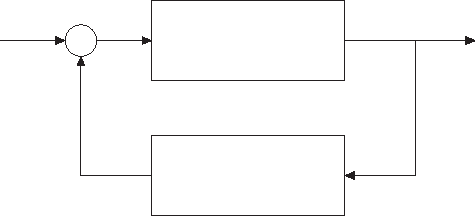
\includegraphics[width=0.5\textwidth]{fnsi/fnsi_feedback}
  \tikzstyle{block} = [draw, fill=white, rectangle, minimum height=3em, minimum width=6em]
  \tikzstyle{sum} = [draw, fill=white, circle, node distance=1.5cm, plus]
  \tikzstyle{input} = [coordinate]
  \tikzstyle{output} = [coordinate]
  \begin{tikzpicture}[auto, node distance=2cm,>=latex']
    \node [input, name=input] {};
    \node [sum, right of=input] (sum) {};
    \node [block, right=1cm of sum, align=left] (system)
      {Underlying linear\\ system: $\bm M, \bm C, \bm K$};
    \node [output, right=2cm of system] (output) {};
    \node [block, below of=system, align=left] (feedback)
      {Nonlinear feedback:\\ $c_a, \bm g_a(\bm y(t), \dot{\bm y}(t))$};
    \draw [draw,->] (input) -- node {$\bm p(t)$} (sum);
    \draw [->] (sum) -- node {} (system);
    \draw [->] (system) -- node [name=y] {$\bm y, \dot{\bm y}$}(output);
    \draw [-] (y) |- (feedback);
    \draw [->] (feedback) -| node [near end] {} (sum);
  \end{tikzpicture}
  \caption{Feedback interpretation of nonlinear structural dynamics.}
  \label{fig:fnsi_feedback}
\end{figure}


Using the state vector $\bm x = [\bm y, \dot{\bm y}]^T$, the system
\eqref{eq:EOM_fnsi_final} is rewritten as the state space formulation
\begin{equation}
  \label{eq:fnsi_c_state_space}
  \begin{split}
    &\dot{\bm x}(t) = \bm A_c \bm x(t) + \bm B_c \bm e(t) \\
    &\bm y(t) = \bm C \bm x(t) + \bm D \bm e(t)
  \end{split}
\end{equation}
where subscript $c$ denotes {\textit continuous time}. $\bm e(t) =
[\bm p(t)^T, g_1, \dots , g_s]^T \in \mathbb{R}^{n+s}$ is the extended input
vector which concatenates external and nonlinear terms.

State-space and physical matrices have the relations
\begin{equation}
  \label{eq:state_to_physical_mat}
  \begin{gathered}
  \bm A_c =
  \begin{bmatrix}
    \bm O  & \bm I \\
    -\bm M^{-1}K     & -\bm M^{-1} \bm C \\
  \end{bmatrix}
  \\
  \bm B_c =
  \begin{bmatrix}
    \bm 0 & \bm 0 & \bm 0 & ... & \bm 0 \\
    \bm M^{-1}  & -\mu_1 \bm M^{-1} \bm b_1 & -\mu_2 \bm M^{-1} \bm b_2 & ... &
    -\mu_s \bm M^{-1} \bm b_S \\
  \end{bmatrix}
  \\
  \bm C =
  \begin{bmatrix}
    \bm I & \bm 0
  \end{bmatrix}
  \,\quad
  \bm D = \bm 0
\end{gathered}
\end{equation}
The state matrices are: $\bm A$ and $\bm B$ the input and nonlinear coefficients
matrix, the output matrix $\bm C$ and the direct feed through matrix $\bm D$.

Before Fourier transforming the system, a continuous to discrete-time conversion
of the state matrices are used with the sampling frequency $f_s$. This is done
in order to improve the numerical condition and given by
\begin{equation}
  \begin{gathered}
    \bm A_d = \text{expm}(\bm A_d/f_s) ,\quad
    \bm B_d = (\bm A_d - \bm I)\bm A_c^{-1} \bm B_c \\
    \bm C_d = \bm C_c ,\quad \bm D_d = \bm D_c
  \end{gathered}
\end{equation}
It is stressed\autocite{noel2013a} that the conversion is only strictly valid if
the input signals in $\bm e$ are piece-wise constant between sampling instants,
called a zero-order hold intersample assumption. This is generally not the case
but if a sufficiently high sampling frequency is used, the continuous time model
is not affected. It is not clear how high a \textit{sufficiently high sampling
  frequency} is.

Using a discrete Fourier transform, the system is
\begin{equation}
  \label{eq:fnsi_freq_state}
  \begin{aligned}
    z_k \bm X &= \bm A_d \bm X(k) + \bm B_d \bm E(k) \\
    \bm Y(k) &= \bm C \bm X(k) + \bm D \bm E(k)
\end{aligned}
\end{equation}
where $z_k = e^{(2i\pi k/N_s)}$ is the z-transform variable for discrete time
models and $N_s$ the number of recorded samples in the time series. $\bm X, \bm
Y$ and $\bm E$ are the discrete Fourier transforms of $\bm x, \bm y$ and $\bm
e$. The subscript $d$ are dropped in the following, as all operations are on
discrete time models.

\subsection{The output-state-input equation}

The extended input $\bm E$ and output $\bm Y$ are known. The system matrices $\bm
A$ and $\bm B$ needs to be determined. As seen from eq.
\eqref{eq:state_to_physical_mat} $\bm C$ and $\bm D$ are known, but are still
estimated as part of the subspace method. These estimates of course match the
known values.

Frequency-domain subspace methods estimates these matrices based on a
reformulation of the state-space eqs. \eqref{eq:fnsi_freq_state} in matrix form,
where the input and output is rearranged into Hankel-type block matrices.

The matrix of the measured output spectra is

\begin{equation}
  \bm Y_i =
  \begin{bmatrix}
    \bm Y(1) & \bm Y(2) & \dots & \bm Y(F) \\
    z_1\bm Y(1) & z_2\bm Y(2) & \dots & z_F\bm Y(F) \\
    z^2_1\bm Y(1) & z^2_2\bm Y(2) & \dots & z^2_F\bm Y(F) \\
    \vdots \\
    z^{i-1}_1\bm Y(1) & z^{i-1}_2\bm Y(2) & \dots & z^{i-1}_F\bm Y(F)
  \end{bmatrix}
\end{equation}
which by defining $\xi = \text{diag}(z_1, z_2, \dots, z_F)$ is recast to

\begin{equation}
  \bm Y_i =
  \begin{bmatrix}
    \bm Y^T & (\bm Y \xi)^T & \dots & (\bm Y \xi^{i-1})^T
  \end{bmatrix}^T
\end{equation}
and similar the matrix of extended input spectra is formed as
\begin{equation}
  \bm E_i =
    \begin{bmatrix}
      \bm E^T & (\bm E \xi)^T & \dots & (\bm E \xi^{i-1})^T
    \end{bmatrix}^T
\end{equation}
where $i$ is a user-defined number of block rows in $\bm Y_i$ and $F$ the number
of frequency lines used for identification; more on how these are chosen later.

Introducing the extended observability matrix
\begin{equation}
  \bm \Gamma_i =
  \begin{bmatrix}
    \bm C^T & (\bm C \bm A)^T & \dots & (\bm C \bm A^{i-1})^T
  \end{bmatrix}^T
\end{equation}
and the lower-block triangular Toeplitz matrix

\begin{equation}
  \bm H_i =
  \begin{bmatrix}
    \bm D                   & \bm 0                   & \bm 0                   & \dots & \bm 0 \\
    \bm C \bm B             & \bm D                   & \bm 0                   & \dots & \bm 0 \\
    \bm C \bm A \bm B       & \bm C \bm B             & \bm D                   & \dots & \bm 0 \\
    \vdots \\
    \bm C \bm A^{i-2} \bm B & \bm C \bm A^{i-3} \bm B & \bm C \bm A^{i-3} \bm B & \dots & \bm D
  \end{bmatrix}^T
\end{equation}
then by recursive use of eq. \eqref{eq:fnsi_freq_state} and the above matrices
\autocite{noel2013a}, the output-state-input matrix equation, which is used for
estimation in the subspace method, is obtained
\begin{equation}
  \label{eq:fnsi_state_matrix}
  \bm Y_i = \bm \Gamma_i \bm X + \bm H_i \bm E_i
\end{equation}


\subsection{Estimation of state matrices}

The subspace method is applied to eq. \eqref{eq:fnsi_state_matrix} in order to
estimate $\bm \Gamma_i$. When $\bm \Gamma_i$ is estimated, the state matrices of
eq. \eqref{eq:fnsi_freq_state} are extracted and calculated.

The method have two main steps:
\begin{itemize}
\item Eliminate the term depending on nonlinearities and forces in eq.
  \eqref{eq:fnsi_state_matrix}, ie $\bm H_i$ by its inclusion of $\bm B$. This
  is done by projecting the equation onto the orthogonal complement of $\bm
  E_i$,
  \begin{equation}
    \bm Y_i / \bm E_i^\perp = \bm \Gamma_i \bm X / \bm E_i^\perp +
    \underbrace{\bm H_i \bm E_ / \bm E_i^\perp}_{=0}
    = \mathcal{P}
  \end{equation}
  The geometrical interpretation of this is shown in figure
  \ref{fig:fnsi_geometric} for the 2d case.

  $\Gamma_i$ is then estimated from a singular value decomposition(SVD) of the
  projection $\mathcal{P}$
\item When $\Gamma_i$ is estimated, the four state space matrices ($\bm A, \bm
  B, \bm C, \bm D$) are calculated.
\end{itemize}

See figure \ref{fig:fnsi_methodolgoy} for a overview.

\begin{figure}[!ht]
  \centering
  \def\svgwidth{6cm}
  \import{fig/fnsi/}{fnsi_geometric2.pdf_tex}
  \caption{Geometric interpretation of eq. \eqref{eq:fnsi_state_matrix} in two
    dimensional space. The orthogonal complement of $\bm E_i$, $\bm E_i^\perp$,
    is the set of all vectors that are orthogonal to every vector of $\bm E_i$
    (thus it is also the null space of $\bm E_i$).
    In the 2d case, $\bm E_i^\perp$ is simply the vector perpendicular to $\bm
    E_i$, and the projection of $\bm Y_i$ onto $\bm E_i^\perp$ cancels the
    extended input term $\bm H_i \bm E_i$. }
  \label{fig:fnsi_geometric}
\end{figure}


\begin{figure}[!ht]
  \centering
  \begin{mdframed}
    \begin{enumerate}
    \item Choose the index $i$ and the number of processed frequency lines $F$
    \item Concatenate external forces and nonlinearities to form the extended
      input spectra $\bm E_i$
    \item Compute the orthogonal projection
      \begin{equation*}
        \mathcal{P} = \bm Y_i / \bm E_i^\perp
      \end{equation*}
      using QR-decomposition.
    \item Compute the SVD of $\mathcal{P}$
      \begin{equation}
        \label{eq:fnsi_svd}
        \mathcal{P} = \bm U \bm S \bm V
      \end{equation}
    \item Determine model order $n$ from singular values in $\bm S$ or from a
      stabilisation diagram. Truncate $\bm U$ and $\bm S$ accordingly to define
      $\bm U_1$ and $\bm S_1$.
    \item Estimate the extended observability matrix $\bm \Gamma_i$
      \begin{equation*}
        \hat{\bm \Gamma}_i = \bm U_1 \bm S_1^{1/2}
      \end{equation*}
    \item Estimate $\bm A$ using the shift property of $\bm \Gamma_i$,
      \begin{equation*}
        \underline{\bm \Gamma_i} \hat {\bm A} = \overline{\bm \Gamma_i}
        \iff
        \hat {\bm A} = \underline{\bm \Gamma^+_i} \overline{\bm \Gamma_i}
      \end{equation*}
      where $\underline{\bm \Gamma_i}$ and $\overline{\bm \Gamma_i}$ are the
      matrix $\bm \Gamma_i$ without its first and last $l$ rows.
      $\bm C$ is extracted as the first block row of $\bm \Gamma_i$.
    \item Estimate $\bm B$ and $\bm D$ by defining the extended FRF  $\bm
      H^e(k)$ (or as this within the $z$-transform it might be termed
      \textit{transfer function}).
      \begin{equation*}
        \bm H^e(k) = \bm C(z_k \bm I - \bm A)^{-1} \bm B + \bm D
      \end{equation*}
      and minimise the difference between the measured and modelled output
      spectra in a linear least square sense, i.e.
      \begin{equation*}
        \hat {\bm B}, \hat {\bm D} = \arg \min_{\bm B, \bm D} \sum_{k=1}^F |\bm Y(k) - \bm H^e(k) \bm E(k)|^2
      \end{equation*}
    \item Convert $\bm A, \bm B, \bm C$ and $\bm D$ into continuous-time
      matrices and form the extended FRF $\bm H^e(\omega)$.
      \begin{equation}
        \label{eq:extend_FRF_He}
        \bm H^e(\omega) = \bm C_c \left(j \omega \bm I^{n \times n} - \bm A_c \right)^{-1} \bm B_c + \bm D_c
      \end{equation}
    \item Estimate the nonlinear coefficients $\mu_j$ and the linear FRF matrix
      $\bm H(\omega)$.
      The FRF matrix of the underlying linear system $\bm H(\omega)$ and the
      nonlinear coefficients $\mu_s$ are found from \eqref{eq:extend_FRF_He} as
      \begin{equation}
        \label{eq:FRE_H}
        \bm Y(\omega) = \bm H(\omega)
        \begin{Bmatrix}
          \bm I & -\mu_1\bm b_1 & ... & -\mu_s \bm b_s
        \end{Bmatrix}
        \bm E (\omega)
        =
        \bm H^e(\omega) \bm E(\omega)
      \end{equation}
    \end{enumerate}
  \end{mdframed}
  \caption{Overview of the FNSI methodology}
  \label{fig:fnsi_methodolgoy}
\end{figure}

Three assumptions are assumed to be fulfilled for the subspace methods,
\begin{enumerate}
\item All the linear modes of vibration in the frequency band of interest are
  excited or, alternatively, they are all observable in input-output data.
\item The row space of the states $\bm X$ and of the extended input spectra
  matrix $\bm Y_i$ does not share information,
  \begin{equation*}
    \text{span}_{\text{row}} (\bm X) \cap \text{span}_{\text{row}}(\bm E_i) = 0
  \end{equation*}
\item The extended inputs $\bm E_i$ are of full rank, i.e.,
  \begin{equation*}
    \text{rank}(\bm E_i) = (s+n) i
  \end{equation*}
  eg. excitations and the nonlinearities have to be such that the inversion of the
  problem is well-posed.
\end{enumerate}

To expand on the second assumption:
The state term $\bm A \bm X$ contains linear stiffness and damping information.
If constant and/or linear terms are introduced in the nonlinear basis functions,
the intersection between the states and the extended inputs $\bm E_i$ is no
longer empty, which violate the assumption.
This requires nonlinear basis functions to be nonlinearisable.

\FloatBarrier


\subsection{Types of nonlinear basis functions}
\label{sec:fnsi_functional}


As stated, the nonlinear basis functions should be zero and have zero slope at
the origin. For continuous nonlinear restoring force, polynomial functions with
order chosen from WT- and RFS plots can be used. For discontinuous systems, e.g.
contact, polynomials might not be well suited; higher order polynomials might
exhibit oscillations around the origin. An alternative is to use piecewise cubic
spines instead. Even if they cannot realise a perfect fitting (they are
continuous by nature), they are appropriate for representing sudden events, like
sharp changes in stiffness(or damping) curves. Cubic splines and polynomials can
be mixed. See section \ref{sec:contact_identification} for the formulation
needed for using splines.

Using cubic splines might be termed \textit{gray box} identification where using
polynomials is \textit{white box}. The difference is that with gray box, the
nonlinearities are described by functions that may represent a vast variety of
nonlinear behaviour and thus requiring less specific knowledge of the underlying
physics.


\subsection{Estimating model order}

In order to do parameter estimation, the number of block rows $i$ in the Hankel
matrices, used frequency lines $F$ and the model order $n$ must be chosen by the
user.
There is no strict way to chose $i$, the only requirement is that it is chosen
greater than the system order $n$. In theory the larger $i$, the more accurate
estimation (which is true until a given limit, where the repeated inclusion of
the system dynamics affects the conditioning). In practice the identification is
not that sensitive to the value of $i$, but a too large value impact the
computational time.

The frequency lines $F$, ie. the frequency content to include in the estimation,
are often chosen as the same as the excitation frequency band. If the structure
is excited with a $0-150$Hz band, $F$ could be chosen as $5-150$Hz, neglecting
low-level and \textit{out-of-input-band} frequencies. Or chosen as the
frequencies around resonances of the system, neglecting the frequencies with low
throughput. The reason for truncating the frequencies are to save computational
time.

The model order $n$ is strictly the number of total linear modes of the system
eq. \eqref{eq:EOM_fnsi}, but in practice only a limited set modes are excited
during measurement. Thus to determine $n$, is equal to determine the number of
modes excited in the chosen frequency interval $F$.
This means that stabilisation diagram can be used to determine $n$ instead
of inspecting the singular values of $\bm S$, eq. \eqref{eq:fnsi_svd}.

To calculate a stabilisation diagram, the linear modal parameters are estimated
for a given model order, ie. natural frequency, damping and mode shape. These
modal parameters are then compared to the modal parameters calculated using a
\textit{one higher} model order.
Comparing modal parameters for each identified mode of the two model orders then
gives the stability: \textit{stabilisation in frequency}, \textit{stabilisation
  in damping} and \textit{stabilisation of the mode shape}. If all three
parameters are stabilised the mode is full stabilised. The natural frequencies
and damping are compared to some tolerance chosen by the user and stabilisation
of the mode shape is calculated by the modal assurance
criterion(MAC)\autocite{Allemang2003},

\begin{equation}
  MACX(r,q) = \frac{|\bm \psi^T_r \bm \psi^*_q|^2}
  {\left( \bm \psi^T_r \bm \psi^*_r \right)\left( \bm \psi^T_q \bm \psi^*_q \right)}
\end{equation}

% For simulated data without noise, tolerances for frequency, damping and mode
% stabilisation are $0.5\%, 2\%, 0.98$ respectively.


If the model order is chosen too low, it will result in unmodelled dynamics,
whereas too large order lead to overmodelling issues such as an increase of the
noise sensitivity of the model. It should be noted that model selection requires
that adequate basic functions are used.

Without anticipating the example, a stabilisation diagram for the coupled
duffing system is shown in figure \ref{fig:fnsi_stab} along with singular values
of $\bm S$ in figure \ref{fig:fnsi_svg}. The two modes are clearly seen.
From the stabilisation diagram a model order of four is chosen. This gives
stabilisation in the linear parameters. The plot of the singular values shows a
jump of six orders magnitude between model order four and five, verifying the
chosen model order.
In general only the stabilisation diagram is used as it gives more detailed
information; the singular value plot is only used if a stabilisation diagram is
not implemented.

\begin{figure}
  \centering
  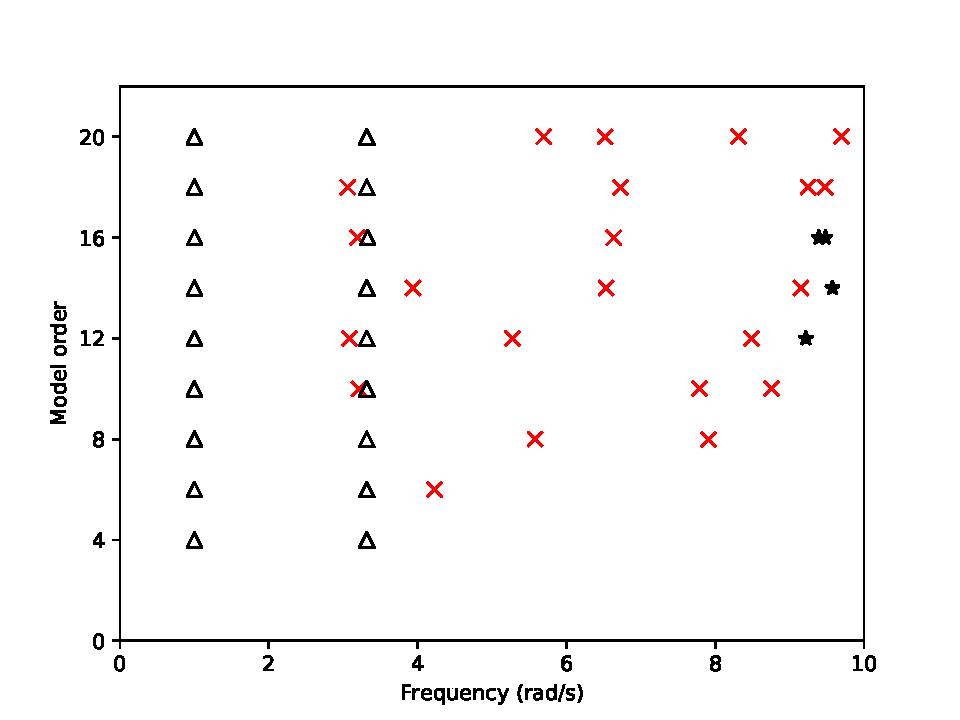
\includegraphics[width=0.8\linewidth, height=8cm]{fnsi/vrms3_stab}
  \caption{Estimation of model order. Stabilisation diagram with linear FRF
    overlayed. Two modes are identified.
    \textcolor{red}{$\pmb\times$}: new natural frequency(termed pole);
    $\pmb\star$: stabilisation in natural frequency;
    % $\pmb\square$: extra stabilisation in damping ratio;
    % $\pmb\circ$: extra stabilisation in MACX;
    $\pmb\triangle$: full stabilisation.
    Stabilisation thresholds in natural frequency, damping ratio and MACX value
    are $0.5\%, 2\%, 0.98$, respectively.
  }
  \label{fig:fnsi_stab}
\end{figure}

\begin{figure}
  \centering
  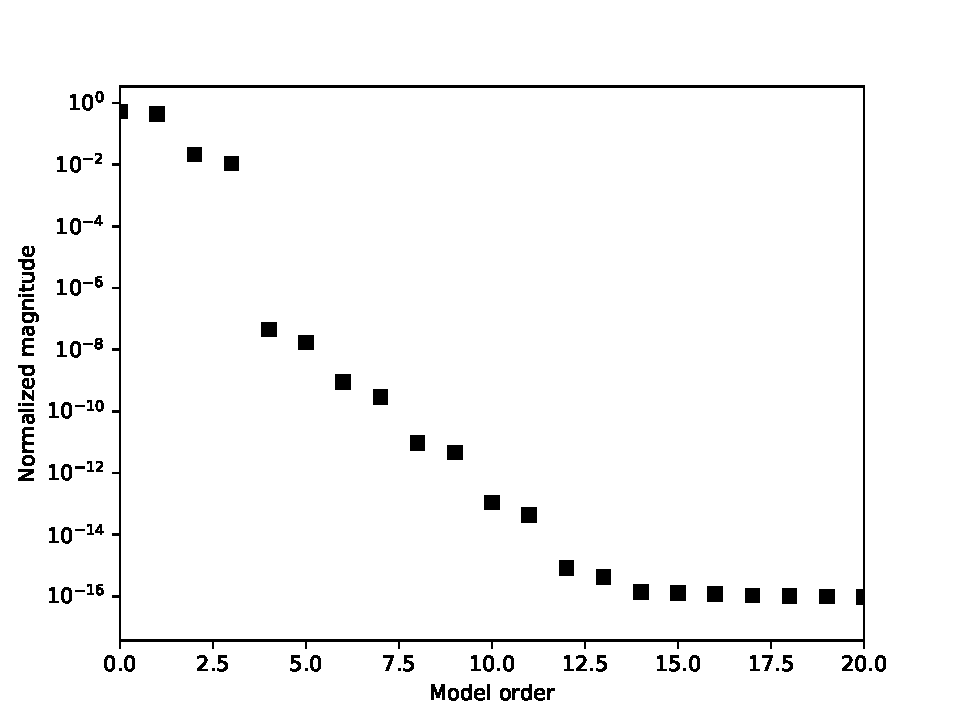
\includegraphics[width=0.6\linewidth, height=6cm]{fnsi/vrms3_svg}
  \caption{First twenty singular values. A jump of six orders magnitude is seen
    between model order four and five.}
  \label{fig:fnsi_svg}
\end{figure}

The determination of the model order is very simple and clear here. For larger system this
might not be the case, see \autocite{noel2014a} for an example.


\subsection{Example}
\label{sec:fnsi_example}

The coupled duffing system is excited with a periodic multisine a integer
number times. Using a periodic signal a integer number of times should avoid
leakage\autocite{ewins2000a}.
Figure \ref{fig:periodicity} shows the periodicity of the recorded signal. The
periodicity is calculated by using the signal of the last period as a reference
and then subtracting this reference from each of the previous periods. If the
difference between the reference and a previous period is close to zero, often
shown in a logarithmic scale, the periodicity between the reference and the
compared period is low. Ie. the periodicity is a way to verify that transient
effects are died out.

To summarise; for estimation multiple periods can be used, but transient effects
should not be present; which is indicated by a low periodicity. In this case
periods 4-9 could be used.

\begin{figure}[!ht]
  \centering
  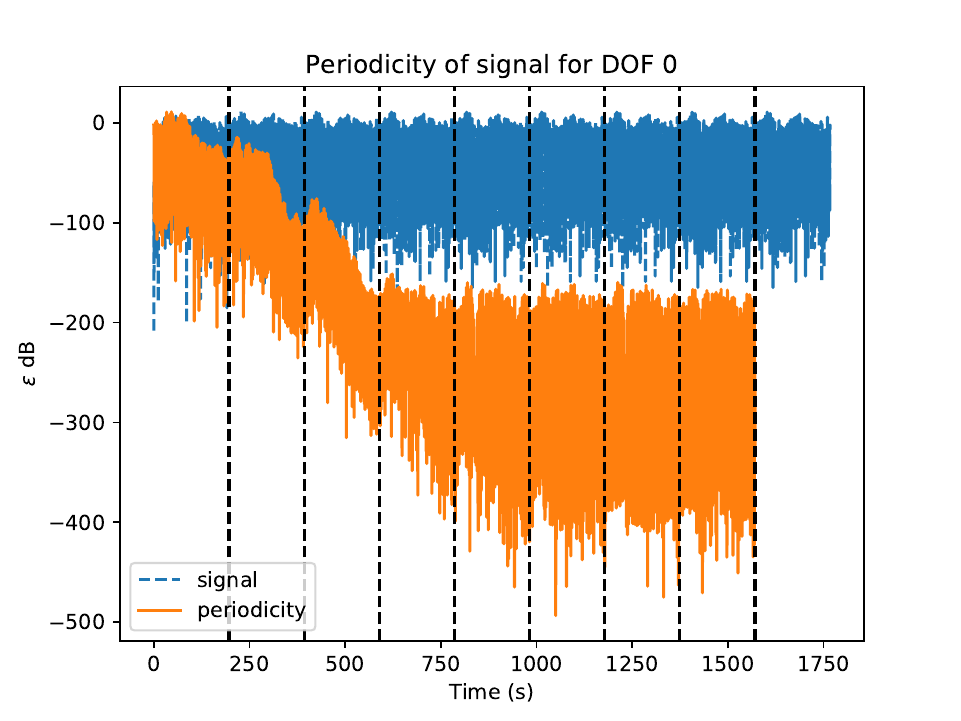
\includegraphics[width=0.7\linewidth]{fnsi/frf_per.png}
  \caption{Periodicity (or difference between periods) of recorded signal at DOF
    0. Vertical lines indicate periods. A low periodicity shows that transient
    effects have died out. Blue is the original signal and yellow the
    periodicity.}
  \label{fig:periodicity}
\end{figure}


The estimation of the nonlinear parameters of the system is shown in figure
\ref{fig:fnsi_knl} for model order four. The variation of the real part of $\mu$
is shown in a 1\% interval, with very little frequency dependency in the
frequency range of interest. The imaginary part is about three orders of
magnitude smaller. Both indicates a good quality of the estimation. The spectral
averages are
\begin{equation}
  \begin{aligned}
    \Re (\mu_1) = 1.000, \quad \Im (\mu_1) = 1.09 \times 10^{-4} \\
    \Re (\mu_2) = 1.000, \quad \Im (\mu_1) = 7.73 \times 10^{-4}
  \end{aligned}
\end{equation}
and matching the simulated values well.

\begin{figure}[!ht]
  \centering
  \begin{subfigure}[b]{0.45\textwidth}
    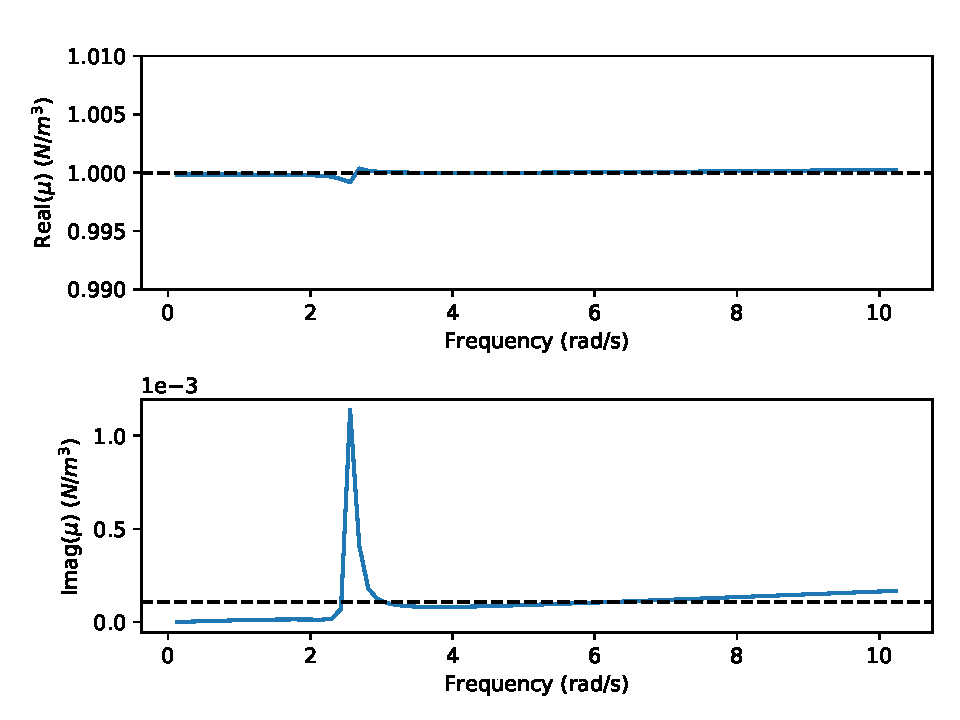
\includegraphics[width=\linewidth]{fnsi/vrms3_knl0}
    \caption{}
  \end{subfigure}
  ~
  \begin{subfigure}[b]{0.45\textwidth}
    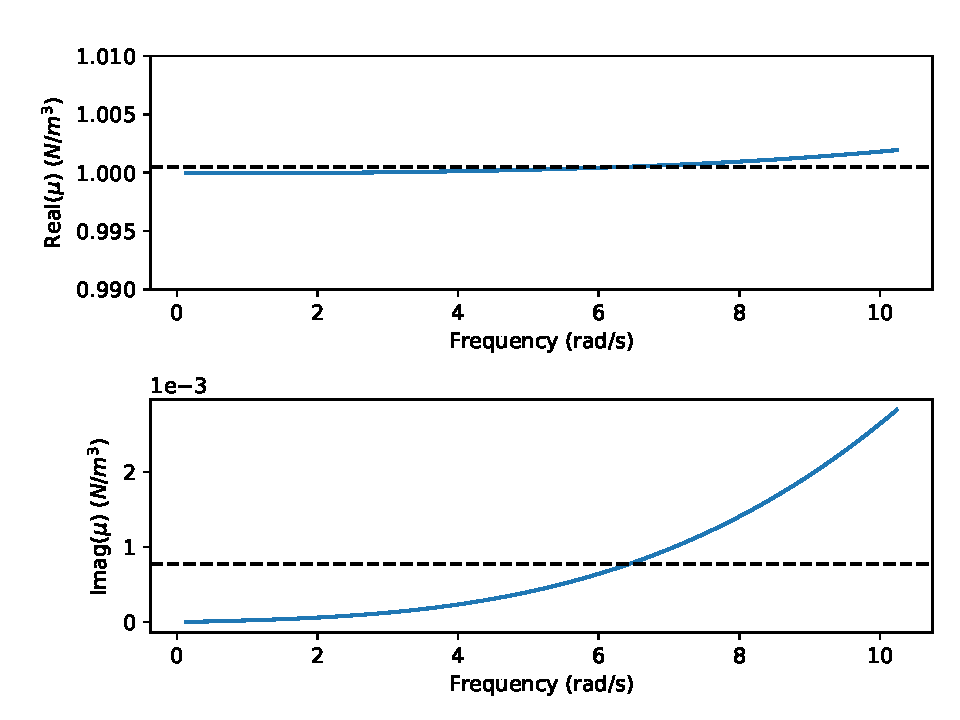
\includegraphics[width=\linewidth]{fnsi/vrms3_knl1}
    \caption{}
  \end{subfigure}
  \caption{Real and imaginary part of estimated nonlinear coefficients $\mu_1$
    and $\mu_2$. The variation of Re($\mu$) is shown in a 1\% interval, with
    very little frequency dependency in the frequency range of interest.
    The imaginary part is about three orders of magnitude smaller. Both
    indicates a good quality of the estimation.
    \textbf{(a)}: $\mu_1$;
    \textbf{(b)}: $\mu_2$.
  }
  \label{fig:fnsi_knl}
\end{figure}

The FNSI method also estimate the underlaying linear properties. As seen from
table \ref{tab:fnsi_eigen}, the linear parameters are identified correctly.
Ensuring that linear parameters are identified, also shows that nonlinear
coefficients are identified correct.

\begin{center}
  \begin{tabular}{*{3}{c}}
    \hline
    Mode & Frequency (rad/s) & Damping ration (\%) \\
    \hline
    1 & 1.00 & 5.00 \\
    2 & 3.32 & 1.51 \\
    \hline
    1 & 1.19 & 3.96 \\
    2 & 3.40 & 1.41 \\
    \hline
  \end{tabular}
  \captionof{table}{Estimated linear natural frequencies and damping ratios for
    the coupled Duffing system.
    \textbf{(upper)}: Nonlinear identification with FNSI;
    \textbf{(lower)}: Linear identification
  }
  \label{tab:fnsi_eigen}
\end{center}

Figure \ref{fig:fnsi_H1} shows the FRF. The linear FRF found by FNSI match the
theoretical linear FRF.

\begin{figure}[!ht]
  \centering
  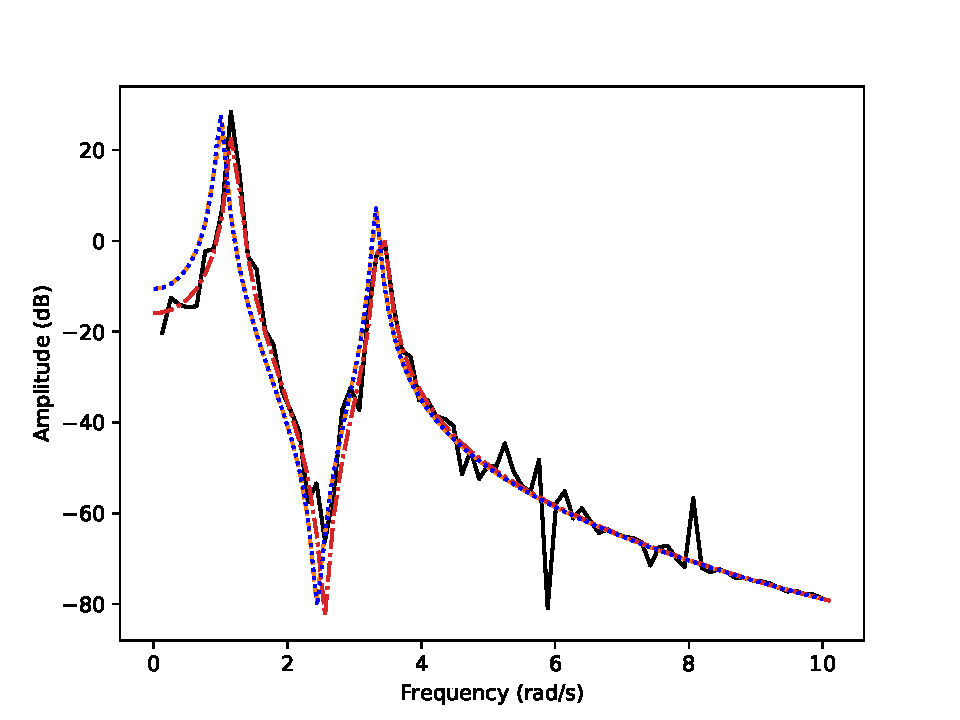
\includegraphics[width=0.8\linewidth, height=10cm]{fnsi/vrms3_H1}
  \caption{FRF calculated as $H_1$ for the coupled duffing system.
    \sampleline{}: H1 from signal;
    \textcolor{red}{\sampleline{dash pattern=on .7em off .2em on .2em off .2em}}: Linear identified;
    \textcolor{orange}{\sampleline{dashed}}: Nonlinear identified from FNSI;
    \textcolor{blue}{\sampleline{dotted}}: Theoretical linear
    % \sampleline{dash pattern=on .7em off .2em on .05em off .2em}
  }
  \label{fig:fnsi_H1}
\end{figure}

\subsection{Estimation error}
\label{sec:fnsi-estimation-error}

It seems that the FNSI method works quite well - both nonlinear and linear
parameters are estimated with high accuracy - as seen from the simple example
and in a broader sense:~\autocites{noel2013a, noel2014a, noel2014b,
  noel2012time}.

However as shown in \autocite{gourc2016a} spurious terms appears in the
estimated $\bm B_c$ matrix. These terms have only limited affect on the
estimated parameters, but if the estimated state space matrices are used
directly for simulation purposes, ie. coupling a numerical continuation method
directly with the state space model to obtain a NFRC without building a FE
model, the spurious terms does affect the location of resonance peaks as they
are acting as damping.

The spurious terms in $\bm B_c$ arise from the conversion between discrete- and
continuous time. As stated, the identification is done in discrete time, but the state space
model is used in continuous time.
To quote J.P Noel, who introduced FNSI, from a mail correspondence:
\begin{quote}
The continuous-time models are well suited for mechanical applications. The reason
for this is that continuous-time identification assumes that data are acquired
in band-limited conditions, i.e. that the input and the output are only
measured over a finite set of frequencies, which is always the case in a
mechanical setup. However, from a numerical point of view, it is more stable to
carry out the identification in discrete time which is done, knowing that this
creates an error.
\end{quote}

A final remark is that the state space matrices are not found within a basis for
the physical coordinate system, ie. wrt. to the vector basis $\bm x=[\bm y^T,
\dot{\bm y}^T]^T$. It was not mentioned in the overview fig.
\ref{fig:fnsi_methodolgoy}, but the estimation of the extended observability
matrix $\bm \Gamma$ is done within a similarity transformation matrix $\bm
T$, ie.
\begin{equation}
  \bm \Gamma = \bm U_1 \bm S_1^{1/2} \bm T
\end{equation}
where the similarity transform is chosen as $\bm T = \bm I$ and thus omitted in
successive steps. But this fixes the state-space basis and as the nonlinear
components of $\bm B$ changes with the basis, they cannot be extracted from $\bm
B$ by using a similarity transform changing the basis to physical coordinates.
This is the reason why the nonlinear coefficients have to be extracted from the
invariant extended FRF $\bm H^e$ and not simply found by inspection of $\bm B$.

Without any explanation it is stated the similarity transform
\begin{equation}
  \bm T =
  \begin{bmatrix}
    \hat{\bm C} \\
    \hat{\bm C} \hat{\bm A}
  \end{bmatrix}
  , \quad
  \bm A = \bm T \hat{\bm A} \bm T^{-1}, \quad
  \bm C = \hat{\bm C} \bm T^{-1}
\end{equation}
gives the state matrices $\bm A, \bm C$ in physical space, ie. matching the
formulation eq. \eqref{eq:state_to_physical_mat}. \^{} denotes the estimated
matrices.

% Another reason for the difficulty
% To demonstrate this, it is noted that the state space matrices are obtained by a
% similarity transformation matrix $\bm T$:
% \begin{equation}
%   \bm A_c = \bm T \hat{\bm A}_c \bm T^{-1}, \quad
%   \bm B_c = \bm T \hat{\bm B}_c, \quad
%   \bm C_c = \hat{\bm C}_c \bm T^{-1}, \quad
%   \bm D_c = \hat{\bm D}
% \end{equation}
% where \^{} denotes estimated quantities. Normally $\bm T$ is simply chosen as
% the identity matrix, and thus ignored in the overview fig.
% \ref{fig:fnsi_methodolgoy}, as the nonlinear coefficients are not invariant wrt.
% to

% as the nonlinear coefficients are not extracted directly
% from $\bm B$ but from the invariant extended FRF eq. \eqref{eq:FRE_H}.

% which is why it is not included in the overview of FNSI in
% fig \ref{fig:fnsi_methodolgoy}. As the nonlinear

% but to obtain the
% state-space matrices in physical coordinates, ie. wrt. to the vector basis $\bm
% x=[\bm y^T, \dot{\bm y}^T]^T$

\subsection{Summary}
\label{sec:summary-fnsi}

The FNSI method is able to identifying multiple nonlinear parameters for system
with many DOFs. It differs from time domain methods, with the ability to
truncate measured signals to the frequency intervals of interest making
computations faster for large systems.

Characterisation of the nonlinearity is important to get a good estimation.
If there is limited knowledge about the nonlinearity, cubic splines can be used
instead of polynomials.
In general the following steps can be used to check the validity of the
identification:

\begin{itemize}
\item Check the stabilisation of the first mode.
\item Check the modal parameters compared to linear identification.
\item Check the stability of the nonlinear coefficients versus frequency.
\item Check the magnitude of the imaginary parts of the coefficients.
\end{itemize}


% \begin{table}[h]
% % scale down the table to the textwidth
% \resizebox{\textwidth}{!}{
% %  \begin{tabularx}{\textwidth}{XXX}
%   \begin{tabular}{lll}
%     \hline
%     Property              & TNSI & FNSI \\
%     \hline
%     Domain & Time & Frequency \\
%     MIMO  & Yes & Yes \\
%     Iterative & No & No \\
%     Data exploited & Transient & Steady State \\
%     Data pre-processing & No & DFT \\
%     Frequency-domain data reduction & Not possible & User-selected bands \\
%     Characterization capability & Multiple-term model and {\textit a posteriori}
%                                   discrimination & Identification error criterion\\
%     Stabilization diagram &  Yes & Yes \\
%     Accuracy of the linear parameter estimates   & High, with larger errors on
%                                                    damping ratios & High, with larger
%                                                                     noise variability\\
%     Accuracy of the nonlinear parameter estimates & High, with larger noise variability & High, with larger
%                                                                                           frequency dependence\\
%     Computational burden & Moderate & Low\\
%     \hline
%   \end{tabular}}
%   \caption{Summary of the properties and identification capabilities of the TNSI
%     and FNSI methods, \citet{noel2014a}}
%   \label{tab:tnsi_fnsi_comparison}
% \end{table}


% Question.
% Dear Jean-Philippe,

% I was at your Nolinsys course in september and would like to demonstrate to my
% supervisor, Jon Juel Thomsen, DTU, how you do parameter estimation.
% So following your paper:
%     Method by J.P Noel. Described in article
%     "Frequency-domain subspace identification for nonlinear mechanical systems"
%     http://dx.doi.org/10.1016/j.ymssp.2013.06.034

% I have done steps up till 10, ie. I can estimate/calculate \hat{E, B, C ,D}
% in step 9 but then I don't know what to do about equation (45).
% I have copied t equations, with dimensions, from your article. See the attached pdf.

% So my question is:
% How do I extract H and \mu from eq. 1.2 (45)? I have calculated H^e, but do not
% understand how to proceed.

% Here is a snippet from my code:

% # step 10
% (loop over omegas: I know it is a bit inefficient, this is just to understand your paper.)
% omegas = range(0,100) # just some range of interest
% for idx, omega in enumerate(omegas):
%     He = C.dot(linalg.inv(np.eye(n,dtype=complex)*1j*omega - A).dot(B)) + D
%     # Calculate H, extract mu's and save in matrix
%     H = ?
%     mu[:,idx] = 



% JUST a note:
% I have also looked at your ph.d thesis. There the formulation seems a bit
% different than in the article, ie:
% Q = H [I^(n,n)  -mu_1 * I^(n,n)  ...  -mu_s * I^(n,n)] E = H^e E

% ie. H is just extracted as the first n columns, as you also write.



%%% Local Variables:
%%% mode: latex
%%% TeX-master: "../../report"
%%% End:
